\documentclass{article} 
\usepackage{mathmag}

\usepackage{amsmath,amsthm}     
\usepackage{graphicx}     
\usepackage{hyperref} 
\usepackage{url}
\usepackage{amsfonts} 

\usepackage{multicol}

% draft watermark
%comment or delete this to remove watermark
%===============================
%\usepackage[svgnames]{xcolor}
%\usepackage[
%    text=DRAFT,
%    scale=5,
%    color={[rgb]{1, 0.85, 0.85}}
%    ]{draftwatermark}
%===============================

% NOTE mathmag.sty calls the text fonts. For this template we are using times.sty 
% from the standard LaTeX distribution.

%% IF YOU HAVE FONTS INSTALLED you can use these math fonts to more
%% closely approximate the final product.
%\usepackage{mtpro2}
%\usepackage{mathtime}

\theoremstyle{theorem}
\newtheorem{theorem}{Theorem}

\theoremstyle{definition}
\newtheorem*{definition}{Definition}
\newtheorem*{remark}{Remark}

\allowdisplaybreaks

\makeatletter
\@addtoreset{footnote}{page}
\makeatother

%%%%%%%%%%%%%%%%%%%%%%%%%%%%%%%%%%%%%%%%%%%%%%%%%%
\begin{document}


\title{Population Models of \textit{Minecraft} Sheep}

\author{Evan Freeland\\               %%%% Leave ALL of these as is in your initial submission
\scriptsize The Ohio State University\\    %%%% to allow for double blind reviewing.
               %%%% They should be filled in when you are submitting
evanfreeland@yahoo.com}                      %%%% your final manuscript.

\maketitle

\section{Introduction}
\textit{Minecraft} is an open-world sandbox video game\footnote{Data for this investigation was collected in \textit{Minecraft} Java edition version 1.19.4.}. The game takes place in a procedurally generated world made of cubic voxels, or \textit{blocks}. Among other activities, players can engage in agriculture, including the raising of sheep. 

Players can gather blocks of wool by raising a flock of sheep in a pasture (Figure \ref{fig:pasture_photo}). When a sheep is sheared, they can eat a grass block to immediately regrow their wool. When a grass block is eaten, it converts into dirt, and can regrow if grass spreads from an adjacent grass block.

\begin{figure}
    \caption{A pasture in a meadow, with woolly and sheared sheep, and grass and dirt blocks.}
    \label{fig:pasture_photo}
    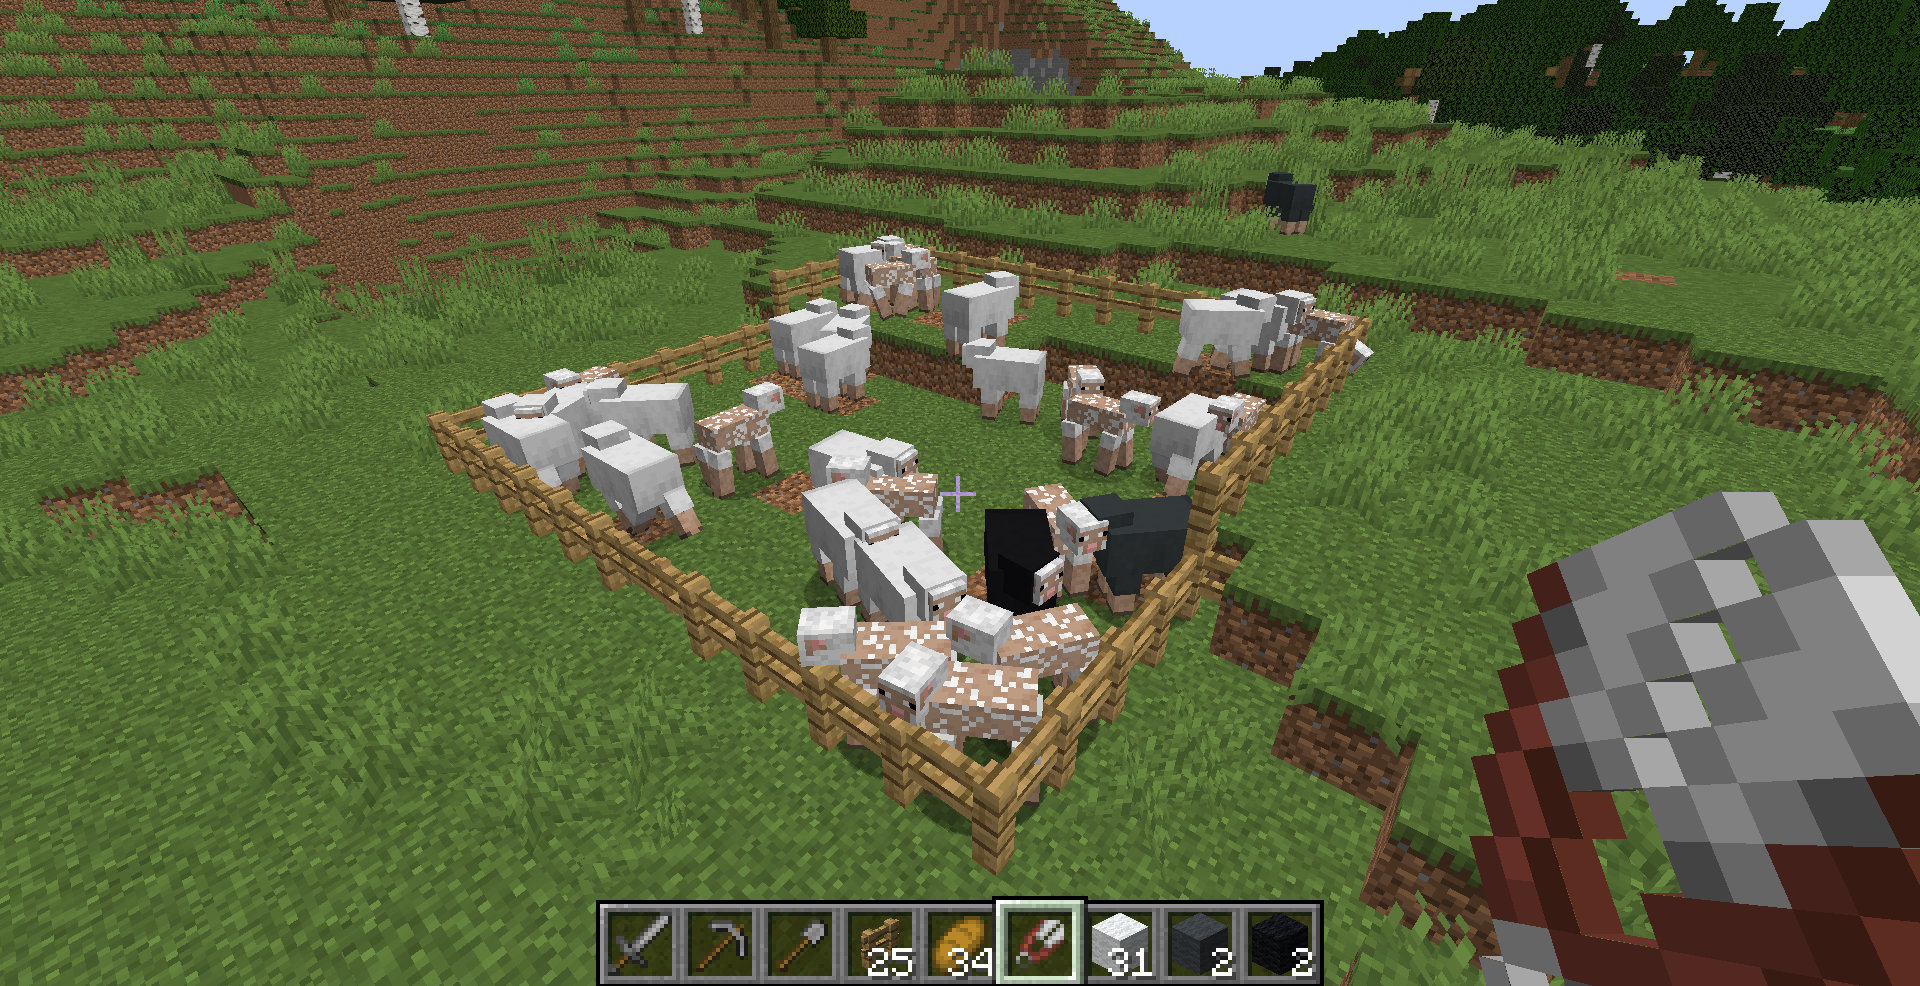
\includegraphics[width=\textwidth]{2023-12-15_22.16.38}
\end{figure}

One may be tempted to pack the pasture as densely as possible to maximize space efficiency. However, if a pasture is packed too densely with sheep, they will deplete the grass, and wool production will be low. On the other hand, if the pasture is not densely packed, wool production will still be low because there are not many sheep. A mathematical population model can give insight into the happy medium sheep population.

\section{Table of symbols}
\begin{center}
    \begin{tabular}{|l|l|l|}
        \hline
        $N$ & Sheep population & sheep\\
        $A$ & Pasture size & blocks\\
        $N_g$ & Grass population & blocks\\
        $\lambda$ & Grass growth rate & blocks s$^{-1}$\\
        $\mu$ & Grass consumption rate & blocks s$^{-1}$\\
        $k$ & Grass growth rate constant & s$^{-1}$\\
        $R$ & Grass consumption rate constant & blocks s$^{-1}$ sheep$^{-1}$\\
        $P$ & Pasture carrying capacity & blocks\\
        $p_x$ & Probability distribution of $N_g$ & \\
        $q_{xy}$ & Probability distribution of $N_g$ and $N_w$ & \\
        \hline
    \end{tabular}
\end{center}

\section{Deterministic model}
\subsection{Grass population}

The \textit{Minecraft} game engine operates in discrete time increments of 0.05 seconds, called \textit{ticks}. Here, this will be approximated as a continuous-time process.

Sheep randomly attempt to eat the block they're standing on. If the sheep and grass in the pasture are uniformly distributed in a pasture with $A$ total blocks, $N_g$ grass blocks, and $N$ sheep, the grass consumption rate $\mu$ is given by
\begin{equation}
    \label{sheep_eat}
    \mu=\frac{NRN_g}{A},
\end{equation}

where $R$ is the frequency with which an individual sheep attempts to eat.

Grass blocks randomly spread to adjacent dirt blocks. If $N_g$ is small, then grass growth will be limited by the lack of places the grass can spread \textit{from}. If $N_g$ is large, grass growth will be limited by a lack of places for the grass to spread \textit{to}. A simple approach is to assume the growth rate $\lambda$ has a parabolic dependence on $N_g$, such that $\lambda=0$ for $N_g=0$ and $N_g=A$ so that
\begin{equation}
    \label{growth_rate}
    \lambda=kN_g-\frac{k}{A}N_g^2,
\end{equation}

where $k$ is a constant related to the rate at which grass spreads.

The overall rate of change of $N_g$ is the difference of $\lambda$ and $\mu$:
\begin{equation}
    \label{logistic}
    \dot{N}_g=\lambda-\mu=\left(k-\frac{NR}{A}\right)N_g-\frac{k}{A}N_g^2.
\end{equation}

This is the \textit{logistic} model \cite{banks}, one of the earliest and simplest models for population growth. It is seldom employed for real-life ecology, having been supplanted by more intricate and flexible models, but it is applicable here due to the simple mechanics of \textit{Minecraft}.

The exact solution of equation \ref{logistic} is
\begin{equation}
    \label{logistic_soln}
    N_g(t)=\frac{P}{1+\left(\frac{P}{N_g(0)}-1\right)e^{-\left(k-\frac{NR}{A}\right)t}},
\end{equation}

where
\begin{equation*}
    P=A-\frac{NR}{k}.
\end{equation*}

The population asymptotically approaches $P$ as $t\rightarrow\infty$. In ecology, $P$ is known as the carrying capacity, the maximum population that a habitat can sustain in equilibrium. This is not to be confused with $A$, the number of blocks in the pasture and therefore the maximum number of grass blocks it can contain. Note also that for $N\geq \frac{Ak}{R}$, the carrying capacity is 0.

\subsection{Experimental determination of rate constants}

The actual values of $k$ and $R$ were determined with in-game experiments. The value of $R$ was measured by counting the number of grass blocks eaten by sheep. In 1 hour, 10 sheep ate 320 blocks of grass, which gives $R=0.00888\mathrm{\;s^{-1}}$.

\begin{figure}
    \caption{Logistic model fit to grass growth data.}
    \label{fig:grass_logistic_fit}
    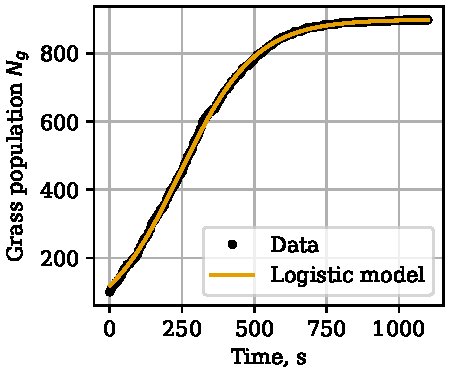
\includegraphics[]{grass_growth/grass_logistic.pdf}
    \centering
\end{figure}

The constant $k$ was measured by uniformly dispersing 100 grass blocks in a 900-block dirt patch and tracking the grass population over time. The grass growth was then fit to equation \ref{logistic_soln}. Figure \ref{fig:grass_logistic_fit} shows the fit of the logistic model to the data collected from the game. This fit gave $k=0.00772\mathrm{\;s^{-1}}$. More details about these experiments can be found on the author's Github\footnote{github.com/ELFREELAND/minecraft\_sheep}.

\subsection{Woolly sheep population}

A naïve assumption is that the farmer has superhuman speed, and shears each sheep the instant it grows its wool. In this case, the rate at which wool is gathered\footnote{Shearing a sheep actually yields between 1-3 blocks of wool, but this is out of the player's control, so it is assumed here that a sheep always yields one wool.} is equal to $\mu$. Denoting the rate of wool gathering with $F$, and substituting $N_g=P$ into equation \ref{sheep_eat} (assuming the pasture has equilibrated),
\begin{equation}
    \label{ffast}
    F=\mu=NR-\frac{N^2R^2}{Ak}.
\end{equation}

This is a simple parabolic relationship with a maximum value of $F=\frac{Ak}{4}$ at $N=\frac{Ak}{2R}$.

A more realistic assumption is that the farmer shears the sheep periodically and at regular intervals. Let $N_w(t)$ be the number of woolly sheep at time $t$. If the farmer shears the sheep with period $T$, the average rate at which they gather wool is
\begin{equation*}
    F=\frac{N_w(T)}{T}.
\end{equation*}

Analyzing this model requires analyzing the evolution of $N_w$ with time. A sheep will only regrow wool upon eating if it doesn't already have any, so one should expect that the rate $\dot{N}_w$ at which sheep regrow wool is proportional to the number $N-N_w$ that are woolless, given by
\begin{equation}
    \label{n_w_dot}
    \dot{N}_w=\frac{N-N_w}{N}\mu=(N-N_w)\frac{RN_g}{A}.
\end{equation}

Solving equation \ref{n_w_dot} with the condition $N_w(0)=0$, and assuming $N_g=P$ (and is therefore time-independent) yields
\begin{equation*}
    N_w(T)=N-Ne^{-TR+\frac{TR^2N}{Ak}},
\end{equation*}

Therefore
\begin{equation}
    \label{fslow}
    F=\frac{N-Ne^{-TR+\frac{TR^2N}{Ak}}}{T}.
\end{equation}

The optimal $N$ can be found by differentiating equation \ref{fslow} with respect to $N$, setting $\frac{dF}{dN}=0$, and solving for $N$. Hence

\begin{equation}
    \left(\frac{TR^2N}{Ak}+1\right)e^{\frac{TR^2N}{Ak}+1}=e^{TR+1},
\end{equation}

at which point we can apply the Lambert $W$ function \cite{corless}, which satisfies \newline$W(xe^x)=x$. This leads to

\begin{equation}
    \label{fslow_optimal_n}
    N=\frac{Ak}{TR^2}(W(e^{TR+1})-1).
\end{equation}

Figure \ref{fig:fslow} shows a plot of equation \ref{fslow}. As $T$ increases, the optimal sheep population also increases, and the optimal rate of wool gathering decreases. Clearly there is a tradeoff between the frequency with which the farmer shears the flock and the rate at which they gather wool.

\begin{figure}
    \caption{Contours of equation \ref{fslow} at constant $T$.}
    \label{fig:fslow}
    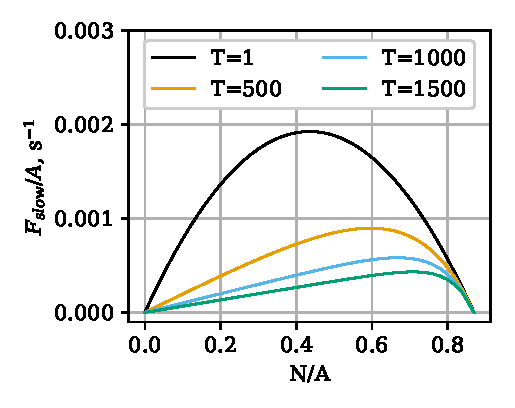
\includegraphics[]{deterministic/f_slow_na_t}
    \centering
\end{figure}

For small $T$, $F$ approximates a parabola. This can be shown quantitatively by employing a first-order approximation for $e^x$, for $x\approx 0$: $e^x\approx x+1$. In equation \ref{fslow}, the exponent is small for small values of $T$, and equation \ref{fslow} reduces to equation \ref{ffast}:
\begin{equation*}
F\approx \frac{N-N(-TR+\frac{TR^2N}{Ak}+1)}{T}=NR-\frac{N^2R^2}{Ak}=\mu.
\end{equation*}

It appears in Figure \ref{fig:fslow} that for large $T$ and small $N$, $F$ is approximately linear with respect to $N$. Under these conditions, all of the sheep have regrown their wool by the time the farmer comes back, and $N_w(T)\approx N$.

\section{Stochastic model}

\subsection{Grass population}
A deterministic model considers population as a single number. A stochastic model considers the \textit{probability distribution} of the population. Here, the grass and sheep will be modelled with a \textit{Markov chain}. The derivation of this method is described in \cite{matis_kiffe}, and applied here for the case of the logistic model.

Let $p_x(t)$ be the probability that the pasture has $N_g=x$ at time $t$. The time derivative of $p_x$ is given by the differential equation
\begin{equation}
    \label{p_dot}
    \dot{p}_x(t)=-p_x(t)(\lambda(x)+\mu(x))+p_{x-1}(t)\lambda(x-1)+p_{x+1}(t)\mu(x+1).
\end{equation}

The first term represents the evolution of the pasture away from $N_g=x$ due to growth or consumption, the second and third terms represent the evolution of the pasture toward $N_g=x$ by growth and consumption, respectively.

Note that $\mu(x)$ simply represnts the value of $\mu$ with $N_g=x$, and likewise for $\lambda$. A pasture of size $A$ will have a system of $A+1$ equations, one for each $x$. Systems of equations such as these, which describe the evolution of a probability distribution with time, are known as \textit{Kolmogorov equations} \cite{matis_kiffe}. In general, Kolmogorov equations can be used to describe a \textit{Markov process}, i.e. a process by which a system transitions between multiple possible states. In this case the states are the possible values of $N_g$.

% \linebreak necessary here because the vector notation will overflow the width

In vector form, this system is expressed as $\dot{\mathbf{p}}(t)=\mathbf{p}(t)\mathbf{R}$, where \linebreak $\mathbf{p}(t)=\left[p_0(t), p_1(t), p_2(t) \dots p_A(t)\right]$, and $\mathbf{R}$ is a matrix of coefficients, such that the coefficient $r_{ij}$ relates $p_i$ with $\dot{p}_j$:
\begin{equation*}
    \dot{p}_j=\sum_{i}r_{ij}p_i
\end{equation*}

\begin{equation*}
    r_{ij}=\begin{cases}
        \lambda(j-1)&\text{for }i=j-1\\
        \mu(j+1)&\text{for }i=j+1\\
        -(\lambda(i)+\mu(i))&\text{for }i=j\\
        0&\text{otherwise}
    \end{cases}
\end{equation*}

This system was solved numerically for pastures of sizes $A=100$, $200$, and $500$, and a range of values of $N$. \textit{Minecraft} pastures typically begin fully covered with grass, so the initial condition will be $\mathbf{p}(0)=[0, 0, 0 \dots 1]$.

Figure \ref{fig:stochastic_Ng} compares the expected value of $N_g$ after 10000 seconds with the deterministic carrying capacity. They line up very closely for small sheep densities, but for large sheep densities, the expected $N_g$ is significantly less than $P$, especially for $A=100$.

\begin{figure}
    \caption{Expected value of $N_g$ at $t=10000$, for $A=100$ and $A=500$. $P$ from the deterministic model is shown as a dotted line.}
    \label{fig:stochastic_Ng}
    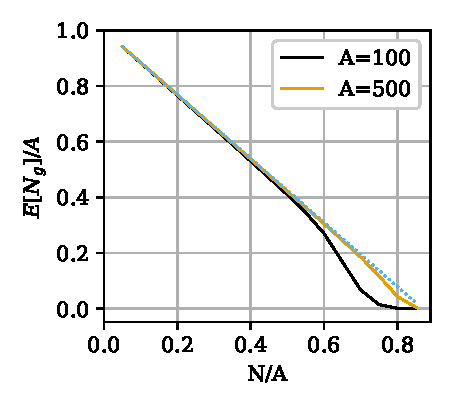
\includegraphics{stochastic/expected_N_g_vs_N}
    \centering
\end{figure}

Figure \ref{fig:evolution} shows the evolution of the distribution of $N_g$ for $N=40$ and $N=70$ in a 100-block pasture. The $N=40$ pasture stabilizes, but the $N=70$ pasture continually evolves toward lower and lower $N_g$, with $p_0$ increasing dramatically as time proceeds.

\begin{figure}
    \caption{Evolution of $N_g$ distribution for a pasture of size $A=100$, for (a) $N=40$ and (b) $N=70$.}
    \label{fig:evolution}
    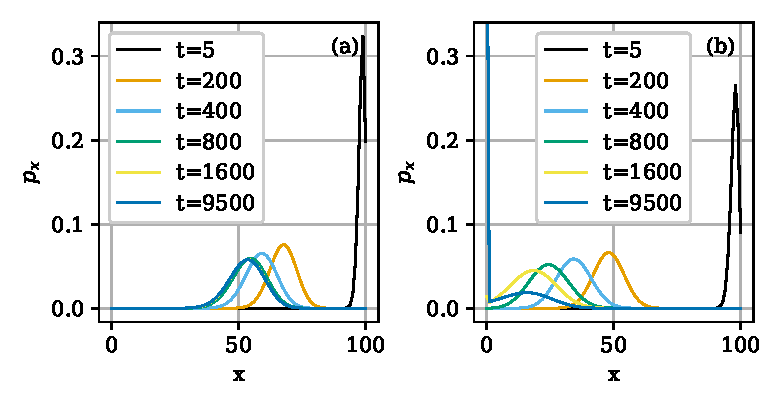
\includegraphics[width=5in]{stochastic/evolution}
    \centering
\end{figure}

The reason for this is evident from the equation for $\dot{p}_0$. Beginning with equation \ref{p_dot} and considering that $p_{-1}=0$ and $\lambda(0)=\mu(0)=0$:
\begin{equation*}
    \dot{p}_0(t)=p_1(t)\mu(1).
\end{equation*}

% \linebreak necessary here too, as above

Since $p_0$ is monotonically increasing, the true equilibrium state is \linebreak $\mathbf{p}=[1, 0, 0, 0, \dots]$ i.e. extinction. However, even if this is the equilibrium state, the pasture may remain at a different \textit{metastable} (or \textit{quasi-equilibrium}) distribution if the probability of extinction remains negligible across reasonable time scales, as seen in Figure \ref{fig:evolution}a.

Rapid grass extinction at high sheep densities poses a problem, since the deterministic model predicts that the optimal $N$ increases as $T$ increases (Figure \ref{fig:fslow}). It can be shown \cite{matis_wehrly_metzler} (see also \cite{matis_kiffe} section 6.8.1.2.) that taking the negative inverse of the coefficient matrix for transient (i.e., nonzero) states, and summing across row $x$ gives the expected extinction time for a starting population of $x$.

Figure \ref{fig:ext_time} shows the expected extinction time, $t_{ex}$, as a function of $N$. For all three pasture sizes, populations close to $\frac{Ak}{R}=0.869$ have extinction time on the order of a few hours. The extinction time increases dramatically, on the order of centuries, with decreasing sheep density and increasing pasture size.

\begin{figure}
    \caption{Expected time to extinction for pastures of $A=100$, $200$, and $500$ as a function of sheep population density.}
    \label{fig:ext_time}
    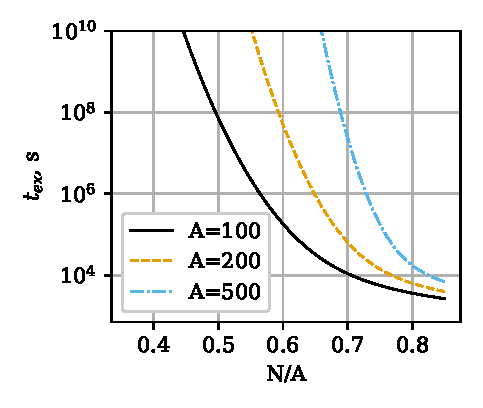
\includegraphics{stochastic/ext_time}
    \centering
\end{figure}

\subsection{Woolly sheep population}

A model for both the sheep and grass mechanics will involve a bivariate probability distribution, $q_{xy}$, where
\begin{equation*}
    q_{xy}(t)=\Pr(N_g(t)=x,N_w(t)=y).
\end{equation*}

Following the same prodecure as with equation \ref{p_dot}:
\begin{equation}
    \label{q_xy_dot}
    \begin{split}
        \dot{q}_{x,y}(t)&=q_{x,y}(t)(-\mu(x)-\lambda(x))\\
        &+q_{x-1,y}(t)\lambda(x-1)\\
        &+q_{x+1,y}(t)\mu(x+1)\frac{y}{N}\\
        &+q_{x+1,y-1}(t)\mu(x+1)\frac{N-(y-1)}{N}.
    \end{split}
\end{equation}

The result is a system of $(A+1)(N+1)$ equations:

$$\dot{q}_{kl}=\sum_{i,j} r_{ijkl}q_{ij}$$

\begin{equation*}
    r_{ijkl}=\begin{cases}
        -\mu(i)-\lambda(i)&\text{for }(i,j)=(k,l)\\
        \lambda(k-1)&\text{for }(i,j)=(k-1,l)\\
        \mu(k+1)\frac{l}{N}&\text{for }(i,j)=(k+1,l)\\
        \mu(k+1)\frac{N-(l-1)}{N}&\text{for }(i,j)=(k+1,l-1)\\
        0&\text{otherwise}
    \end{cases}.
\end{equation*}

As before, this system can be solved numerically. The initial values of $q_{x,0}$ were set using the values of $p_x(t=10000)$ from the grass population model. Figure \ref{fig:fslow_stochastic} shows $F_{slow}$ as calculated from the results of this model. Similar to what we saw in to Figure \ref{fig:stochastic_Ng}, the stochastic model predicts significantly lower $F_{slow}$ than the deterministic model.

\begin{figure}
    \caption{$F_{slow}$ calculated from the stochastic model for sheep and grass, for a pasture with $A=100$. The initial state was obtained from the numerical solution of $p_x$ at $t=10000$.}
    \label{fig:fslow_stochastic}
    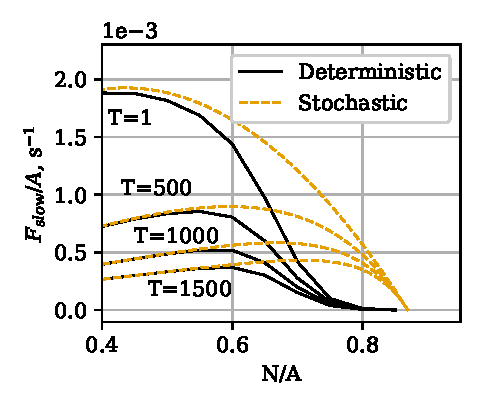
\includegraphics[]{stochastic/fslow_kolmogorov}
    \centering
\end{figure}

The root cause of this deviation is the same as for the grass growth model. The equations for $\dot{q}_{0,y}$ are
\begin{equation*}
        \dot{q}_{0,y}(t)=q_{1,y}(t)\mu(1)\frac{y}{N}+q_{1,y-1}(t)\mu(1)\frac{N-(y-1)}{N}.
\end{equation*}

Since all terms here are positive, $q_{0,y}$ are monotonically increasing, and given enough time, the pasture will tend to evolve into one of these states and never leave.

The biggest drawback of this model is its computational intensiveness. A model for a pasture with $A=500$ and density 0.8 would have $(500+1)(400+1)=200901$ simultaneous equations, and $200901^2=40361211801$ $r_{ijkl}$ coefficients, which would occupy 161 GB of memory if stored as 64-bit floats, making computation infeasable for all but top-shelf consumer hardware.

\section{Conclusions} The logistic model, and the Kolmogorov equations, have proven useful for predicting the behavior of a pasture in \textit{Minecraft}. Other opportunities for modelling video game phenomena include modelling ecomonic phenomena in the \textit{Sims} games, and modelling a virtual disease such as the corrupted blood incident in \textit{World of Warcraft} \cite{lofgren}.

\begin{thebibliography}{1}

    \bibitem{banks} Banks, Robert B. \textit{Growth and Diffusion Phenomena}. Texts in Applied Mathematics. Springer Berlin, Heidelberg, 1994.

    \bibitem{corless} Corless, R. M., G. H. Gonnet, D. E. G. Hare, D. J. Jeffrey, and D. E. Knuth. “On the Lambert W Function.” \textit{Advances in Computational Mathematics} 5, no. 1 (December 1, 1996): 329–59. https://doi.org/10.1007/BF02124750.

    \bibitem{matis_kiffe} Matis, James, and Thomas Kiffe, eds. \textit{Stochastic Population Models: A Compartmental Perspective}. 1st ed. Lecture Notes in Statistics. New York: Springer, n.d.

    \bibitem{matis_wehrly_metzler} Matis, J. H., T. E. Wehrly, and C. M. Metzler. “On Some Stochastic Formulations and Related Statistical Moments of Pharmacokinetic Models.” \textit{Journal of Pharmacokinetics and Biopharmaceutics} 11, no. 1 (1983): 77-92. https://doi.org/10.1007/BF01061769.

    \bibitem{lofgren} Lofgren, Eric T, and Nina H Fefferman. “The Untapped Potential of Virtual Game Worlds to Shed Light on Real World Epidemics.” \textit{The Lancet Infectious Diseases} 7, no. 9 (September 1, 2007): 625-29. https://doi.org/10.1016/S1473-3099(07)70212-8.


\end{thebibliography}

\end{document}